\section{Fire Interpreter}
The fire interpreter's job is to receive input from the simulator and 
calculate values for the received cells. The calculated values are then posted to the visualizer. The advanced regression calculations are done by the library pyXGPR. This is a Gaussian Process Regression library implemented with Python. It produces a mean and a variance when used correctly. The first input parameter \textbf{X} is a list of points which tells where the training data is located. Another parameter \textbf{Y} contains the values to the training data. The last interpreter generated parameter \textbf{x star} contains the points where we want to find the mean and the variance. In addition to these parameters the library needs to be told what covariance functions pyXGPR should use to calculate the correlation between the cells in \textbf{X}, \textbf{Y} and \textbf{x star}. There is also added parameter values to these functions.
\\\\
The most basic use of pyXGPR is one dimensional (line regression) where \textbf{X} is the location and \textbf{Y} is the value. The fire interpreter uses regression in three dimensions where \textbf{x} and \textbf{y} are the map coordinates and an additional parameter \textbf{t} is for time. \textbf{t} is necessary to save earlier sensor data which later are utilized in predictions. It should also be mentioned that before this implementation, this was done by saving the best data. Best data is to be understood as the data which has the lowest variance. Data with lower variance would be applied to the saved map. This hack and the implementation of t is done because previous sensor data is important as long as they are weighted less than the newest sensor data. As time increases there will be sensor data covering a larger portion of the map, but the old sensor data will have less weight and thus giving new sensor data the opportunity to be taken into account. Figure \ref{fig:timeElapse} illustrates this.
\begin{figure}[here]
  \centering
      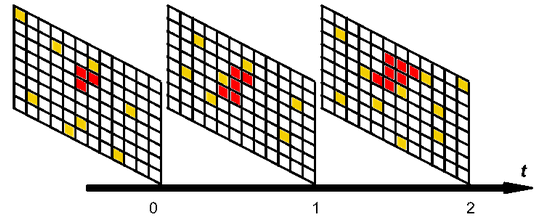
\includegraphics[width=0.5\textwidth]{solution/graphics/timeElapse.png}
  \caption{The fire interpreter saves the sensor data (yellow dots) and gives them a timestamp \textbf{t}. Earlier data is weighted less since the current \textbf{x star} and \textbf{X} has the same and last value for \textbf{t}. }
  \label{fig:timeElapse}
\end{figure}
\subsection{Performance}
The simulation map is 71 X 71 squares. GPR calculates the correlation between all points. This means pyXGPR creates huge matrices. As \textbf{t} increases the matrices grow larger and thus the execution time rises. The first version of the program used more than 6 minutes to run on a normal laptop. To better the performance it was found necessary to locate some squares which did not need to be calculated. Cells containing sensors was therefore removed from \textbf{x star} since the values were already there. With the introduction of \textbf{t}, the matrices became larger and execution time rose and once again it was necessary to find some steps to improve the performance. For a cell to be added to \textbf{x star} it had to be close to sensor which communicated fire. This was done by finding the euclidean distance between all cells which had no value and all sensors which communicated fire. This reduced the number of points in \textbf{x star} significantly. As time increases Another measure taken to reduce the execution time was to save cells which was calculated to be on fire. From these the euclidean distance to all points were calculated and if they were within a certain distance they would be added to \textbf{x star}.
\\\\
Before the interpreter posts the calculated data to the visualizer it converts the mean values to discrete values which is used in the visualizer to decide how intence the fire is burning. A threshold to determine if there should be fire is set, but can be difficult to determine as time progresses. The input values for sensors sensing fire is $0 $ to $10$, while sensors which are not sensing fire is converted from $ 0 $ to $ -1 $. The reason for the conversion is to get some more distance between fire and not fire. The fire threshold is set low to make sure all the realistic fire is covered.
\\\\
\subsection{Changes in pyXGPR kernel to support wind}
The simulation use wind as a crucial parameter to decide where the fire is spreading. Wind is therefore clever to use in the interpretation process. To make it a useful parameter the kernel in pyXGPR has been edited. The kernel contains all the different covariance functions and noise functions. The modification has been done in the function which measures the squared distance between two points. The squared distance is measured by creating two matrices for each dimension. In the fire interpreter these dimensions are \textbf{x}, \textbf{y} and \textbf{t}. One matrix containing all sensor data is deducted from a matrix containing all the uncalculated data. The dimensional result is multiplied with itself and added to a distance matrix. All dimensional results are added to the distance matrix. 
\\\\
\begin{eqnarray}
\theta = cos^{-1}\left(\dfrac{vector_{ij} \times windVector}{\|vector_{ij}\| \times \|windVector\| } \right) 
\label{eq:int-angle}
\end{eqnarray}
\begin{eqnarray}
weight = \dfrac{\theta}{\pi}
\label{eq:weight}
\end{eqnarray}
\begin{eqnarray}
\begin{bmatrix} distance_{11} & distance_{1j} \\ distance_{i1} & distance_{ij} \end{bmatrix} \times 
\begin{bmatrix} weight_{11} & weight_{1j} \\ weight_{i1} & weight_{ij} \end{bmatrix}
\label{eq:hadamard}
\end{eqnarray}
\\\\
Before these calculations the interpreter implementations in this function creates a weight matrix which has the same column and row values as the distance matrix. This weight is calculated with the forumula in \ref{eq:weight}. The Hadamard\cite{hadamard} product (see equation \ref{eq:hadamard}) of these two matrices is returned as the new distance matrix. 
\\\\
Where $ vector_{ij} $ is the vector from sensor position $i$ to uncalculated position $j$. The weight is further normalized to better fit the wind. If $ vector_{ij} $ is between $ 90^{\circ} $ and $ 180^{\circ} $ the weight will be normalized to larger than one and less than one if the angle is less than $ 45^{\circ} $. The values in the weight matrix is multiplied with the values in the distance matrix to create a hadamard\cite{hadamard} product. $ vector_{ij} $ in the weight matrix is multiplied with $ vector_{ij} $ in the distance matrix. This modifies the distance matrix where some values are reduced and some are increased, determined by their vector direction. The correlation of cells looks at the distance between them. Therefore decreased distance to a sensor sensing fire gives a cell a higher probability of being on fire. Sensors which does not detect fire will have a weight of one.
\subsection{Unexpected predictions with wind}
\label{wind-problem}
\begin{figure}[here]
  \centering
      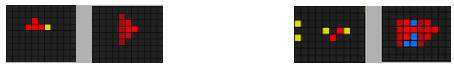
\includegraphics[width=1.0\textwidth]{solution/graphics/wind-problem.png}
  \caption{The left image illustrates when wind is used in predicting fire, while the right image illustrates the faults with a pure wind implementation. The blue dots are where the there should have been predicted fire.}
  \label{fig:wind-problem}
\end{figure}
The implementation of wind is working, but has some drawbacks. The first image in figure \ref{fig:wind-problem} illustrates how the fire is predicted when the wind is blowing from the east. The spread starts where the sensor is located and continuous in the shape of a triangle towards west. This looks good in the first image, but the second image illustrates the drawbacks. The wind is still blowing from the east and the two sensors detecting fire are on a horizontal line. The right tips of the predicted fire is where the sensors are located. The blue squares is used to highlight where there should have been predicted fire. This situation occurs because the blue squares are closest to the second sensor. The vector which goes from the second sensor to the any of blue square has an angle which is more than $ 45^{\circ} $ when compared to the wind vector which is $ \left[-1,0\right] $. Problems with predicting the middle part of the fire can occur when the the size of the predicted fire is becoming quite large. To solve both these problems there has been developed two solutions which have been tested with varying results. The first solution looks at the correlation between all sensors sensing fire while the second solution uses some techniques found in graphical programming. Another approach to these problems would be to use dynamic parameters. As the fire progressed the parameters would change in accordance to the size of the fire. But problems arises with such a solution as well. The edge of the fire would be more likely to be smudged out and it would in some cases predict fire in areas where there were no fire.
\subsubsection{Solution 1 to unexpected predictions with wind}
Burning sensor correlation was one approach to solve the problem when applying wind. It creates a list of all sensors which are sensing fire. Each element in the list has vectors to all other sensors communicating fire. In figure \ref{fig:burning-sensor-correlation} the green triangle is an uncalculated point while the numbered red circles are sensors sensing fire. There are vectors from sensor 1 to all other sensors sensing fire and a vector to the green triangle. This is an illustration of one of the entries in this list. The basis for this theory is that there is probably actual fire between the sensors. The blue vector compares direction with all the black vectors, see \ref{eq:int-angle}. It finds the black vector which has the most similar direction and check if it is within a certain threshold. If this comes out positive the distance for this point to sensor one will be multiplied with a number less than one, else it would be multiplied with one.
\begin{figure}[here]
  \centering
      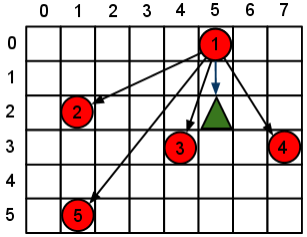
\includegraphics[width=0.4\textwidth]{solution/graphics/burning-sensor-correlation.png}
  \caption{All sensors (red) are sensing fire and sensor one has a vector to all other vectors sensing fire. The green triangle is an uncalculated point. Burning sensor correlation looks for the black vector which has the most similar angle to the closest blue vector.}
  \label{fig:burning-sensor-correlation}
\end{figure}
This approach has a fault. When a situation like \ref{fig:wind-problem} (second image) occurs it would predict fire against the wind. The burning sensor correlation would neutralize the added wind to such a degree that it was removed. The complexity with this solution is high and thus the execution time rises fast as \textbf{t} increases and the fire interpreter uses more data. As this solution was developed it would handle multiple fires badly.
\subsubsection{Solution 2 to unexpected predictions with wind}
In the second approach to solve the wind and filling issues, components from computer graphics were used. The outer boundary of the sensors sensing fire was chosen. The shape will be a convex polygon. Uncalculated cells within this polygon will have a higher probability of being on fire in the prediction. As in the burning sensor correlation implementation it is assumed its a higher probability of being fire between sensors sensing fire.
\begin{figure}[here]
  \centering
      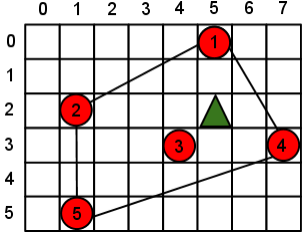
\includegraphics[width=0.4\textwidth]{solution/graphics/graphical-boundary.png}
  \caption{Locates all cells within the boundary.}
  \label{fig:graphical-boundary}
\end{figure}
To locate all the outer cells Graham's scan \cite{graham} was applied. When these points were found Bresenham's\cite{bresenham} line algorithm was used to find the in between cells. The result was all cells which the lines covered in figure \ref{fig:graphical-boundary} was retrieved. After this a scan line fill algorithm was used to find all the cells within the polygon. These steps resulted in a list of cell positions. This list was used when calculating the wind in accordance to wind direction. If the cell to be evaluated was inside this polygon the weight was multiplied with a number lower than one. This solution is also much faster than the first one. The Graham's scan and Bresenham's line algorithm was used as third party code, meaning we did not implement them. But the scan line algorithm was implemented in the kernel. Currently it does not handle multiple fires. If the two fires started at different \textbf{t} it could be possible to walk on predicted fire from one sensor to all the others.
